\chapter{FFDA}
Log-based FFDA di sistemi complessi a larga scala. I dati sono stati collezionati dai supercalcolatori Mercury e Blue-Gene. 
\\Breve descrizione dell'architettura dei due sistemi

La FFDA prevede quattro fasi di sviluppo:
\begin{enumerate}
	\item Data Logging \& Collection. \`{E} una fase che prevede il campionamento dei dati. I dati sono stati già collezionati in automatico sotto forma di file di log (file di testo).
	\item Filtering. Spesso i file di log sono di grosse dimensioni, devono essere opportunamente filtrati per ricavare solo gli eventi interessati. Anche questa fase è già stata effettuata avendo a disposizione gli errori già filtrati.
	\item Manipulation. I dati filtrati devono essere manipolati cercando di individuare e rimuovere gli errori sintomatici della stessa causa.
	\item Data Analisys. Consiste in analisi statistiche sulle informazioni a disposizione con il fine di valutare misure quantitative.
\end{enumerate}
Come già descritto la \textit{fase 1} e la \textit{fase 2} sono già state effettuate.

\section{Manipolazione}
La manipolazione deve essere effettuata per entrambi i supercalcolatori, per cui si ha a disposizione \textit{MercuryErrorLog.txt} (file dei log filtrato di \textit{Mercury}) e \textit{BGLErrorLog.txt} (file dei log filtrato di \textit{BG/L}).
\\La tecnica utilizzata è la \textbf{coalescenza spaziale}. Essa prevede di raggruppare entries preveniente da più nodi diversi, cercando di capire se si sono verificate nello stesso intervallo temporale. Per farlo si utilizza una \textbf{finestra di coalescenza} \textit{W} la quale raggruppa tutte le righe il cui timestamp appartiene a W. Dato che questo valore non è unico, bisogna fare delle analisi solo per sceglierlo.

\subsection{Finestra Temporale}
La finestra di coalescenza viene scelta provando a calcolare il numero di raggruppamenti, che prendono il nome di \textbf{tuple}, per diversi valori di \textit{W}. Si effettua un grafico e si cerca di identificare un "knee", in modo da scegliere quel valore.
\\I tentativi sono stati fatti con i seguenti valori:
\begin{equation*}
	W = \begin{bmatrix}
		10 & 50& 150& 180& 200& 220 \\ 230& 240& 250& 290& 390& 800
	\end{bmatrix}
\end{equation*}
\begin{figure}[H]
	\centering
	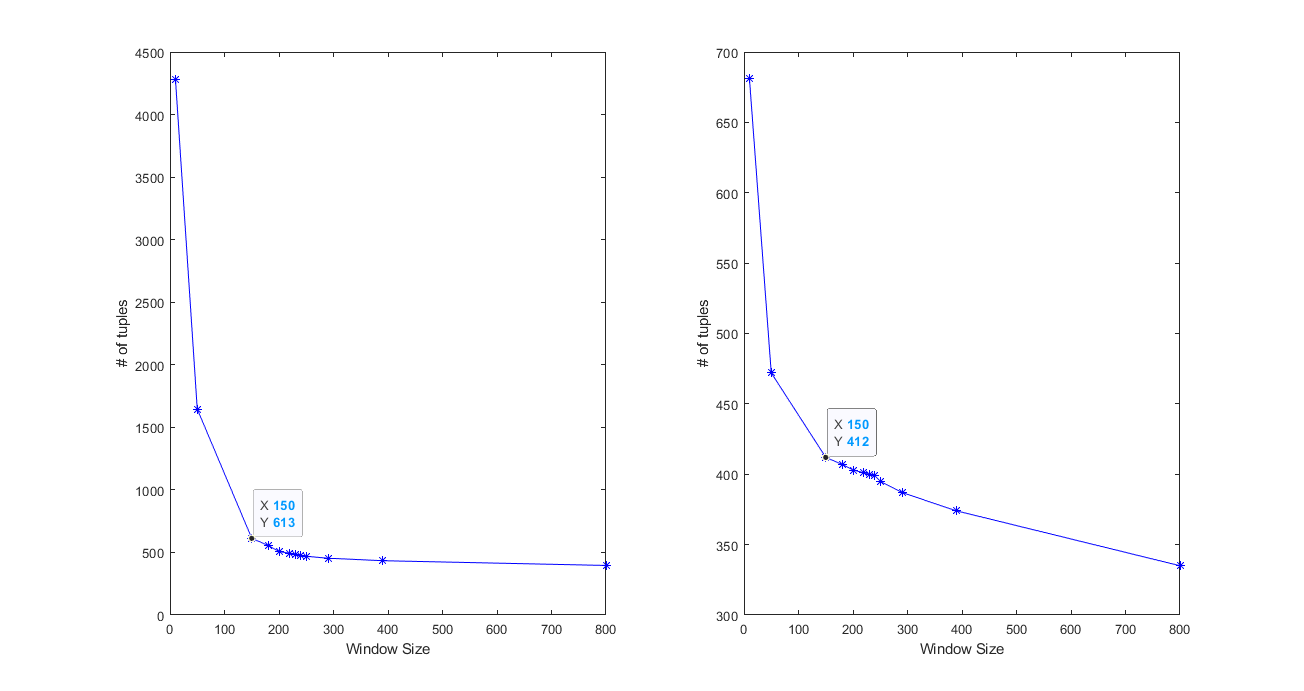
\includegraphics[width=\textwidth]{img/hw6/cwin.png}
	\caption{\textit{Calcolo della Finestra Temporale}}
\end{figure}

Dai grafici si nota che il ginocchio si trova, per entrambi, in corrispondenza di una finestra temporale di \textit{150 secondi}. 
\\Dopo aver deciso \textit{W} per entrambi i log, si possono dividere fisicamente le tuple in file diversi, ognuno quindi può essere analizzato in modo isolato. Per farlo si può utilizzare lo script \textbf{bash} messo a disposizione nel materiale \textit{tupling\_with\_Cwin.sh} il quale prende il ingresso il percorso del file e la finestra \textit{W}.
\\Questo tipo di approccio presenta diverse problematiche, come ad esempio:
\begin{itemize}
	\item \textbf{Troncamento}. L'avvenimento di un \textit{fault} può generare diversi errori che vengono poi collezionati all'interno del file di log. La suddivisione in tuple potrebbe troncare le righe corrispondenti ad uno stesso fault, andandole a dividere, e inserire, in tuple diverse. 
	\item \textbf{Collisione}. Analogamente in una stessa tupla potrebbero comparire eventi che in realtà corrispondono a fault differenti.
\end{itemize} 

\subsection{Analisi del Troncamento}
Un modo semplice per individuare la presenza di possibili troncamenti, è quello di calcolare l'intervallo temporale tra l'ultimo elemento di una tupla e il primo della tupla successiva. Se infatti il tempo di distacco è relativamente basso allora si può pensare che c'è stato un troncamento.
\\Tale informazione temporale viene memorizzata all'interno di un file \textit{interarrivals.txt}, generato dopo la creazione delle tuple con lo stesso script usato precedentemente.
\\Un modo per visualizzare graficamente i possibili troncamenti è quello di porre sull'asse delle x le tuple che si vanno a considerare, e sull'asse delle y il numero di troncamenti conteggiati fino a quella tupla. Per conteggiare un troncamento si può porre un limite di differenza temporale tra una tupla e un altra.
\\Il tutto è meglio descritto con il seguente script MATLAB:
\begin{minted}[framesep = 1mm,
	fontsize = \footnotesize,
	breaklines,
	]{MATLAB}
limit = 2*150;
interarrivi_mercury = load("tupling_MercuryErrorLog-150/interarrivals.txt");
interarrivi_bgl = load("tupling_BGLErrorLog-150/interarrivals.txt");

%% Mercury
j = 1;
hold on;
for i=1:length(interarrivi_mercury)
	if(interarrivi_mercury(i) <= limit)
		tronc_mercury(j) = i;
		plot(i,j, '-*b');
		j = j+1;
	end
end
grid;
xlabel("# di tuple");
ylabel("Numero di troncamenti");

%% BGL
figure;
j=1;
hold on;
for i=1:length(interarrivi_bgl)
	if(interarrivi_bgl(i) <= limit)
		tronc_bgl(j) = i;
		plot(i,j, '-*b');
		j = j+1;
	end 
end
grid;
xlabel("# di tuple");
ylabel("Numero di troncamenti");
\end{minted}
In cui il limite è posto pari al doppio della finestra temporale calcolata. Quindi si suppone che se una tupla si distacca dalla successiva di un valore inferiore a questo limite, allora è possibile che c'è stato un troncamento.
\begin{figure}[H]
	\centering
	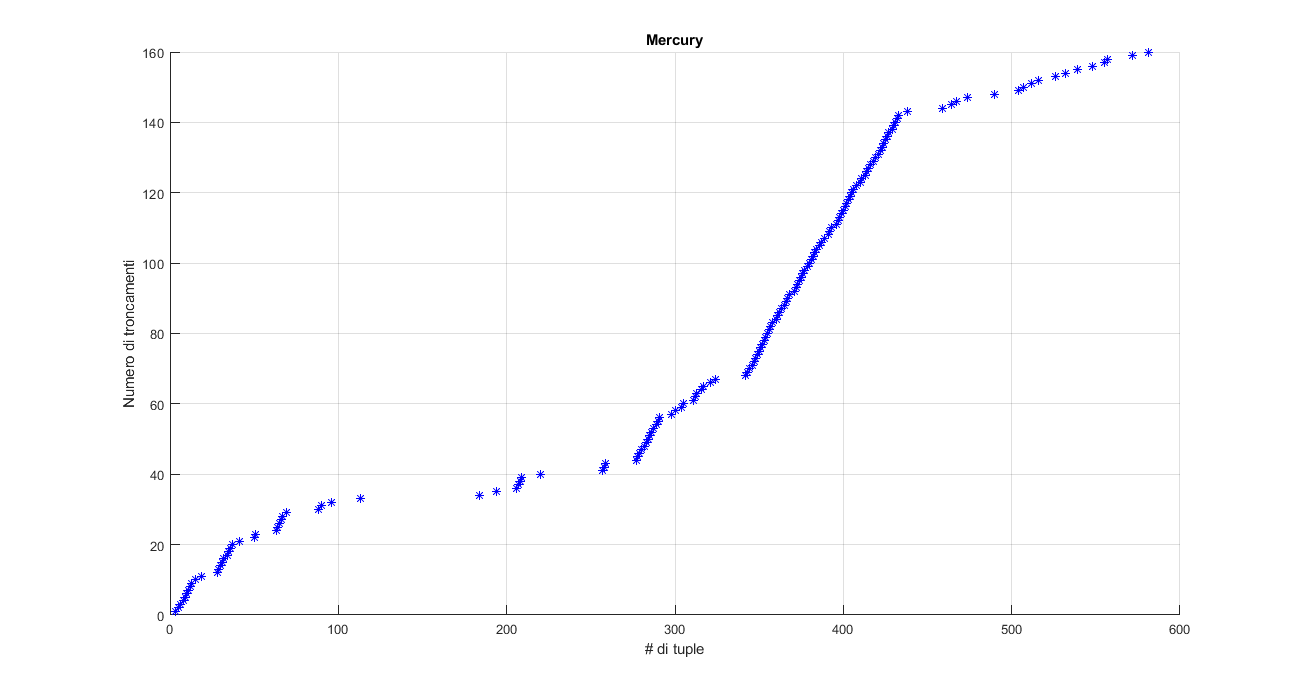
\includegraphics[width=\textwidth]{img/hw6/troncamento_mercury.png}
	\caption{\textit{Numero di troncamenti per tuple}}
\end{figure}
Nel caso Mercury si può notare come tra le tuple 100 e 200 circa, esse si discostano di un valore superiore al limite, portando a pensare che non ci siano stati troncamenti. Al contrario tra le tuple 350 e 400 circa, il numero di troncamenti aumenta velocemente, portando a pensare che in quella finestra temporale i log si riferivano ad uno stesso fault.
\begin{figure}[H]
	\centering
	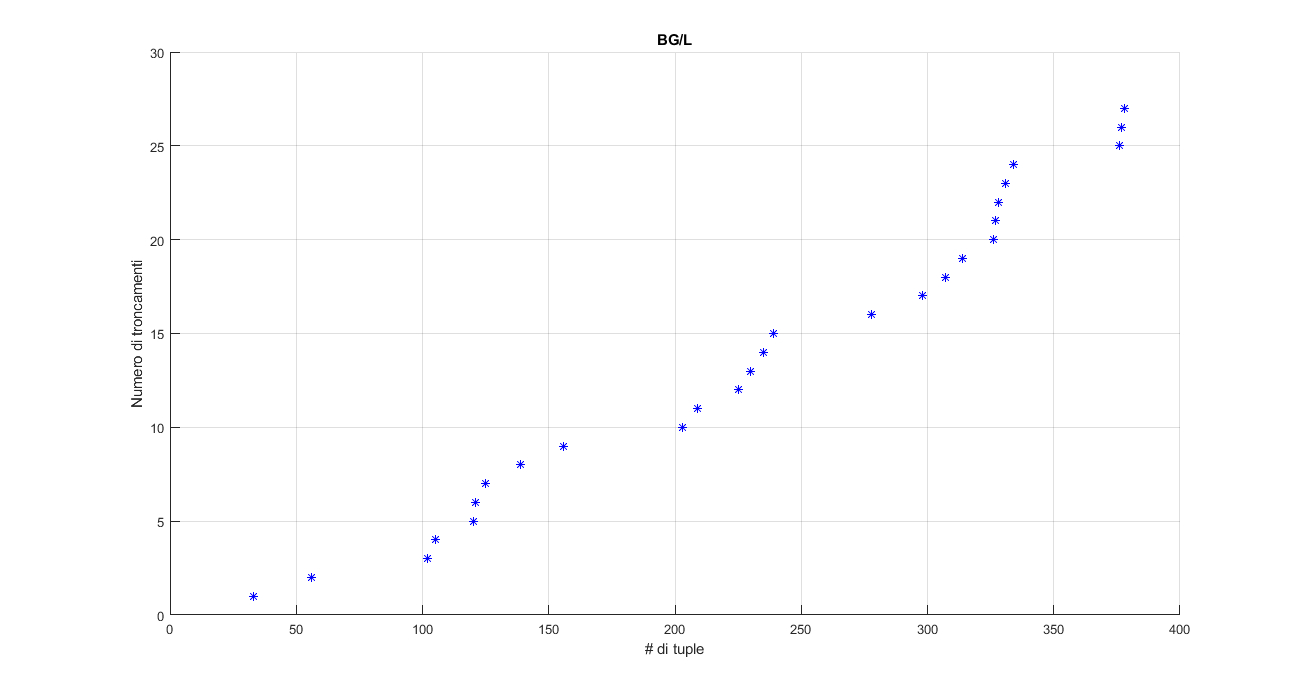
\includegraphics[width=\textwidth]{img/hw6/troncamento_bgl.png}
	\caption{\textit{Numero di troncamenti per tuple}}
\end{figure}
Nel caso di BG/L, invece, il numero di troncamenti sembra essere molto minore; il grafico appare meno denso rispetto a quello di Mercury. 

\subsection{Analisi delle Collisioni}
Le collisioni riguardano fault che innescano errori in più nodi. Bisogna capire dunque se gli errori dei diversi nodi sono stati generati da uno stesso fallimento. Per farlo si analizzano le tuple che presentano errori collezionati da diversi nodi e si cerca di capire se effettivamente essi derivano da uno stesso fault. 
\\Un modo per vedere graficamente la presenza di qualche collisione consiste in:
\begin{enumerate}
	\item Scartare le tuple che hanno all'interno un solo tipo di nodo 
	\item Selezionare una tupla che contiene log riferiti a più nodi
	\item Memorizzare tutti i timestamp della tupla in un vettore
	\item Associare un valore numerico ad ogni possibile nodo del supercalcolatore in esame
	\item Effettuare un grafico tra timestamp e nodo corrispettivo
\end{enumerate}
Quello che ci si aspetta è che ad ogni timestamp viene associato un numero, che corrisponde al nodo corrispettivo. In MATLAB si può realizzare un algoritmo che descrive i passaggi precedenti.
\begin{minted}[framesep = 1mm,
	fontsize = \footnotesize,
	breaklines,
	]{MATLAB}
%% Mercury
N = length(load("tupling_MercuryErrorLog-150/interarrivals.txt")) + 1;
base_path = 'tupling_MercuryErrorLog-150/tuple_';
node_list = [""];
nodes_mercury = [""];
j=1;
k=1;
o=1;
for i=1:N
	path = strcat(base_path,num2str(i, '%d'));
	current_file = fopen(path, 'r');
	while feof(current_file)==0
		row = fgetl(current_file);
		row_splitted = split(row);
		node = row_splitted(2);
		if contains(node_list, convertCharsToStrings(cell2mat(node)))==0
			node_list(j) = convertCharsToStrings(cell2mat(node));
			j = j+1;
		end
		if contains(nodes_mercury, convertCharsToStrings(cell2mat(node)))==0
			nodes_mercury(o) = convertCharsToStrings(cell2mat(node));
			o = o+1;
		end
	end
	if length(node_list) > 1
		file_list_mercury(k) = i;
		k = k+1;
	end
	node_list = [""];
	j=1;
	closeresult = fclose(current_file);
end
\end{minted}
Lo script precedente calcola tutti i nodi che compaiono all'interno del log per Mercury (può essere facilmente adattato per BG/L) e calcola inoltre la lista di file (e quindi le tuple) che contengono più di un nodo.
\\Con tali informazioni basta creare una \textit{map} che associa ad ogni nodo un valore, e effettuare il grafico precedentemente descritto.
\begin{minted}[framesep = 1mm,
	fontsize = \footnotesize,
	breaklines,
	]{MATLAB}
%% Mercury
tupla = 21;

values = 1:length(nodes_mercury);
map_mercury = containers.Map(nodes_mercury,values);

base_path = 'tupling_MercuryErrorLog-150/tuple_';
path = strcat(base_path,num2str(tupla, '%d'));
hold on;
current_file = fopen(path, 'r');
while feof(current_file)==0
	row = fgetl(current_file);
	row_splitted = split(row);
	timestamp = str2num(convertCharsToStrings(cell2mat(row_splitted(1))));
	current_node = map_mercury(convertCharsToStrings(cell2mat(row_splitted(2))));
	plot(timestamp, current_node, '-*b');
end
grid;
xlabel("Timestamp");
ylabel("Nodo");
title("Mercury (tupla 21)");
\end{minted}
Il cui risultato è il seguente.
\begin{figure}[H]
	\centering
	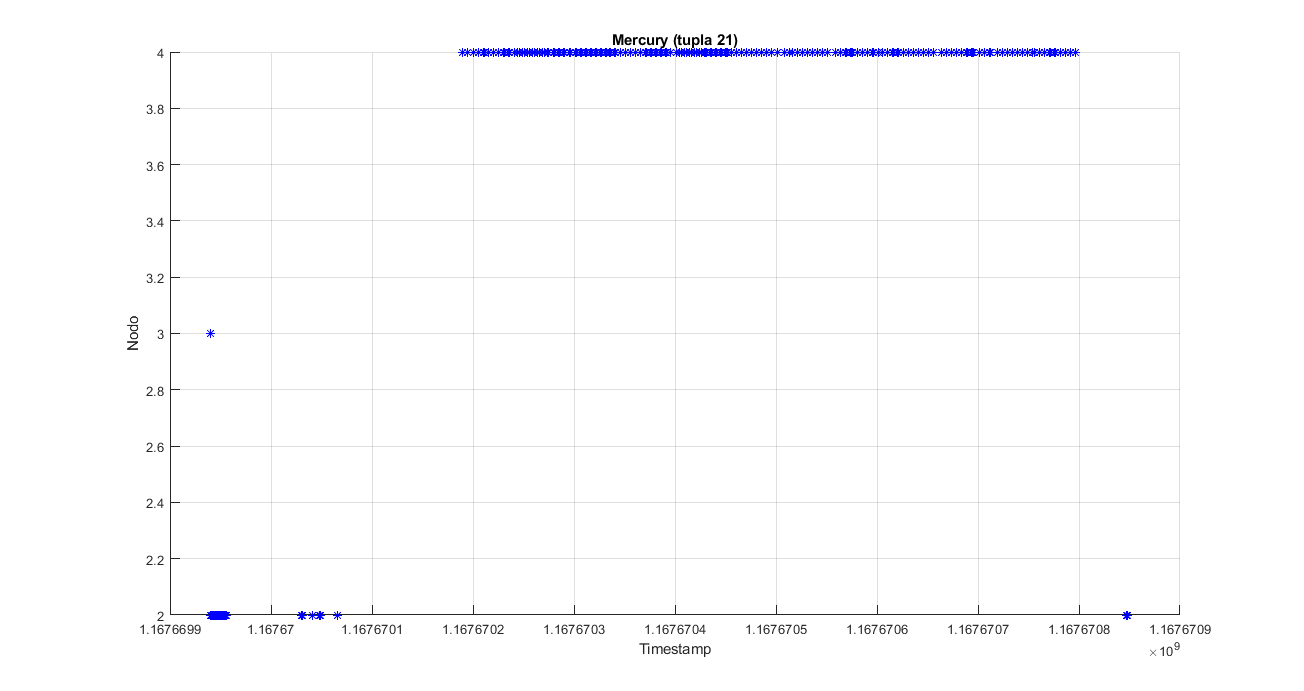
\includegraphics[width=\textwidth]{img/hw6/collisione_mercury.png}
	\caption{\textit{Nodo per timestamp nella tupla 21}}
\end{figure}
Per la tupla in esame, leggendo il grafico, i nodi non si sovrappongono durante la scrittura del log. Questo potrebbe far pensare che non c'è stato un fault che si è propagato tra i nodi.
\\Per BG/L si può effettuare la stessa tecnica.
\begin{figure}[H]
	\centering
	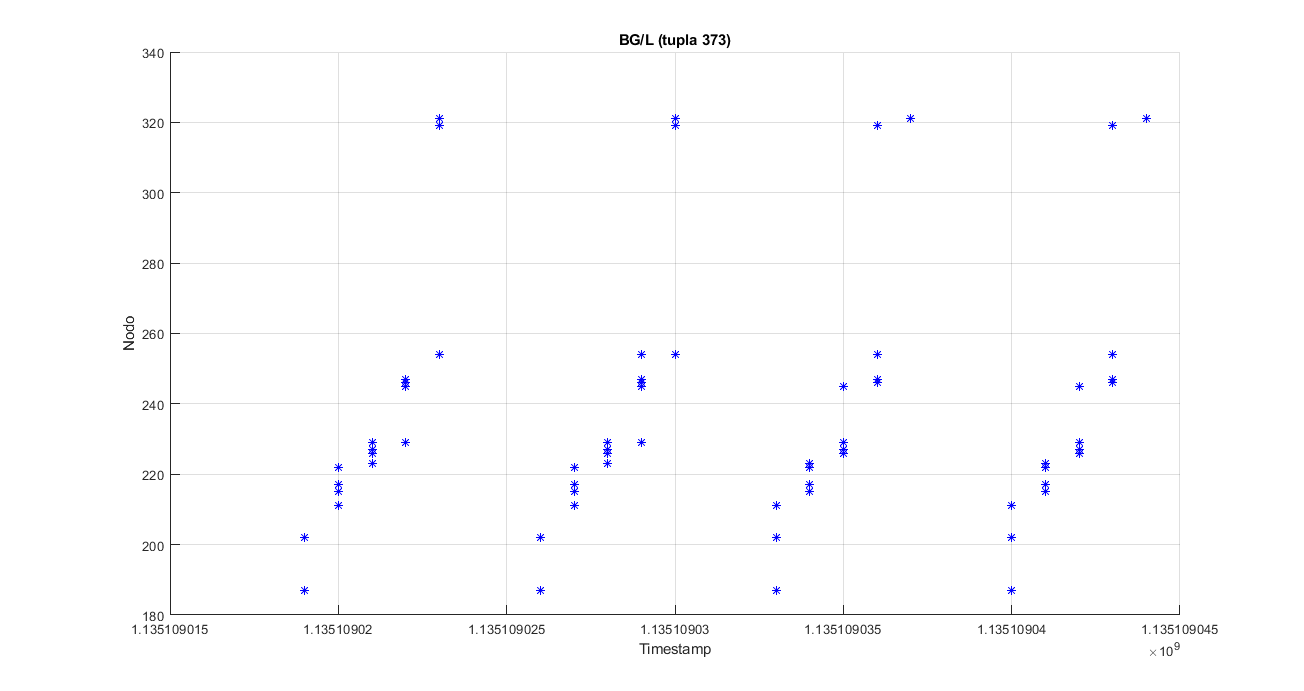
\includegraphics[width=\textwidth]{img/hw6/collisione_bgl.png}
	\caption{\textit{Nodo per timestamp nella tupla 373}}
\end{figure}
Per BG/L si ha un comportamento totalmente diverso. Diversi nodi hanno elaborato un log in un arco di tempo molto breve, andandosi a sovrapporsi tra loro. Inoltre si vede proprio che temporalmente i log sono in successione, portando a pensare che uno stesso fault abbia causato errori nei nodi rappresentati.

\subsection{Domanda 1}
\begin{center}
	\textit{La stessa finestra di coalescenza può essere usata per diversi nodi (fare sia per Mercury che BG) e categorie d'errore (solo Mercury)?} 
\end{center}
Tra il materiale messo a disposizione c'è il file \textit{filter.sh} il quale prende in ingresso un file di log e lo filtra per nodo o categoria d'errore. Quello che si deve fare è effettuare un filtering tre volte:
\begin{enumerate}
	\item Mercury filtrato per Nodo. Sono stati scelti in esame tre nodi:
	\begin{itemize}
		\item \textbf{tg-c401}. Nodo di calcolo
		\item \textbf{tg-login3}. Nodo di login
		\item \textbf{tg-master}
	\end{itemize}
	\item BG/L Filtrato per Nodo. Sono stati scelti anche in questo caso tre nodi:
	\begin{itemize}
		\item \textbf{R12-M0-N0}
		\item \textbf{R63-M0-N2}
		\item \textbf{R71-M0-N4}
	\end{itemize}
	\item Mercury Filtrato per Categoria di Errore. Anche in questo caso sono stati scelte tre categorie:
	\begin{itemize}
		\item \textbf{DEV}
		\item \textbf{MEM}
		\item \textbf{NET}		
	\end{itemize} 
\end{enumerate}
La stessa analisi fatta nella ricerca della finestra di coalescenza deve essere fatta per questi nove nuovi file. 
\\Il risultato per i file di log filtrati per nodo è il seguente:
\begin{figure}[H]
	\centering
	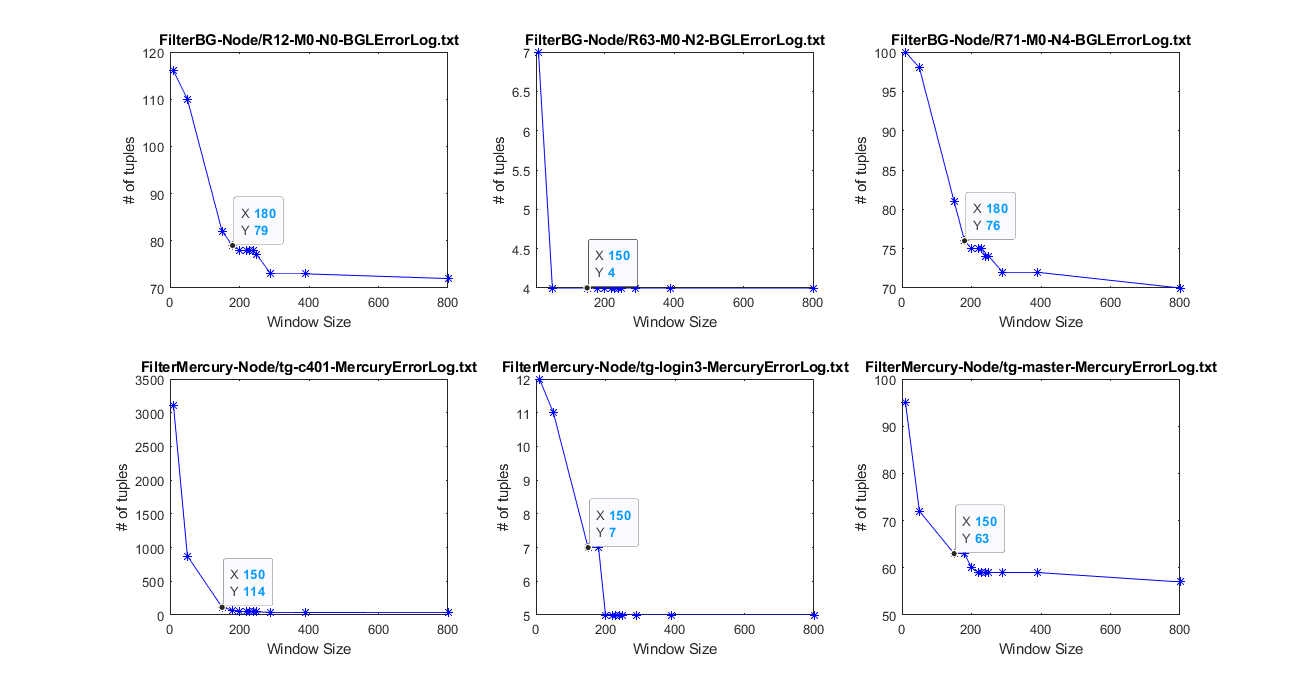
\includegraphics[width=\textwidth]{img/hw6/cwin_mercury_bgl.png}
	\caption{\textit{Calcolo della Finestra Temporale per Nodo}}
\end{figure}
Come si nota dalla figura in grosso modo le finestre temporali sono le stesse del valore \textit{W} scelto per i file di log completi.
\\Il risultato per i file di log filtrati per categoria di errore è il seguente.
\begin{figure}[H]
	\centering
	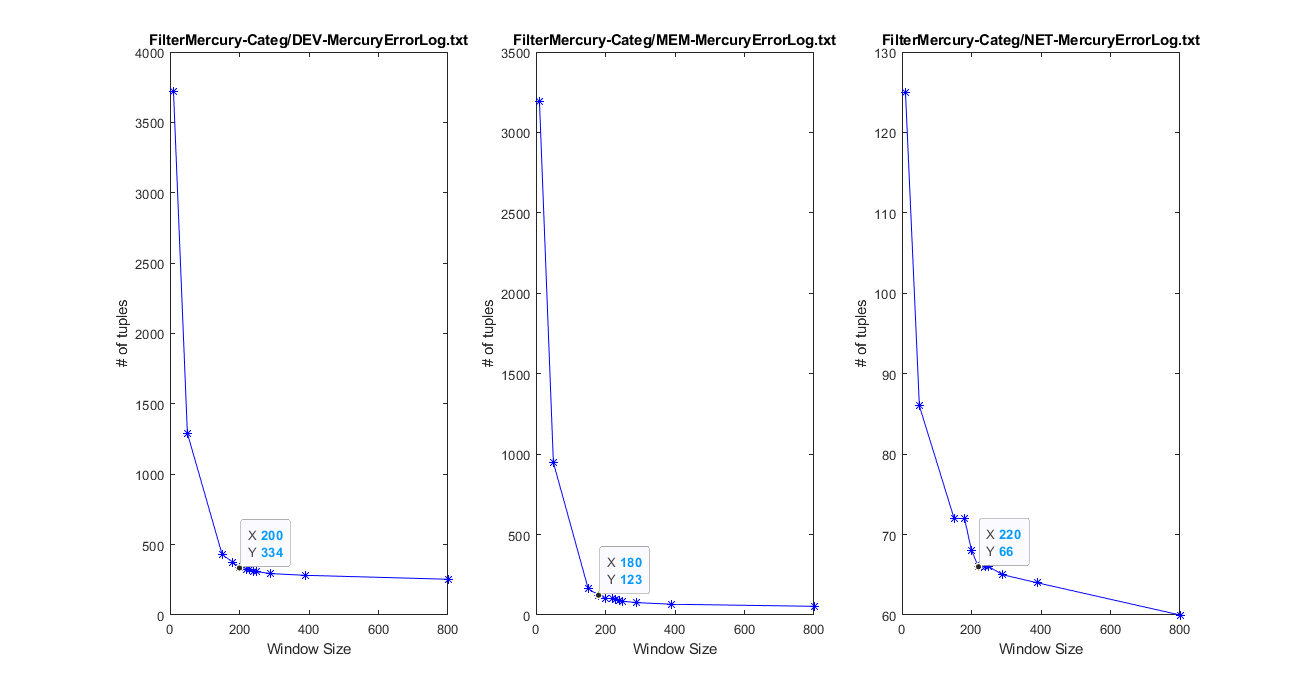
\includegraphics[width=\textwidth]{img/hw6/cwin_mercury.png}
	\caption{\textit{Calcolo della Finestra Temporale per Errore}}
\end{figure}
Anche se nella figura le finestre scelte sono diverse, esse si discostano poco tra loro e soprattutto si discostano poco dal valore \textit{W} scelto nella fase iniziale.


\section{Reliability Modeling}
Una volta ottenuti i dati manipolati è necessario procedere ad una loro analisi. In particolare, si parte dagli \textit{interarrivi} (file interarrivals.txt, ottenuto alla creazione delle tuple), i quali rappresentano la "distanza temporale" tra due tuple consecutive, ovvero il TTF - Time To Failure del sistema complessivo. 
\\L'obiettivo è valutare le distribuzioni empiriche di:
\begin{itemize}
	\item \textit{Tempi di Fallimento - Unreliability},
	\item \textit{Reliability}
\end{itemize}
Con il seguente script MATLAB è stata calcolata la CDF del TTF, e a partire da essa la Reliability empirica del sistema:
\begin{minted}[framesep = 1mm,
	fontsize = \footnotesize,
	breaklines,
	]{MATLAB}
	load interarrivals.txt;         
	[y,t] = cdfcalc(interarrivals); %ne calcolo la CDF = unreliability
	empTTF = y(2:size(y,1));        %scarto la prima riga (?)
	empRel = 1 - empTTF;            %Reliability
	plot(t,empTTF,'-*b');
	hold on;
	plot(t,empRel,'-+r');
	xlabel('time[s]');
	ylabel('p');
	legend('empTTF','empRel');
\end{minted}
\subsubsection{EmpTTF e EmpRel - Mercury}
\begin{figure}[H]
	\centering
	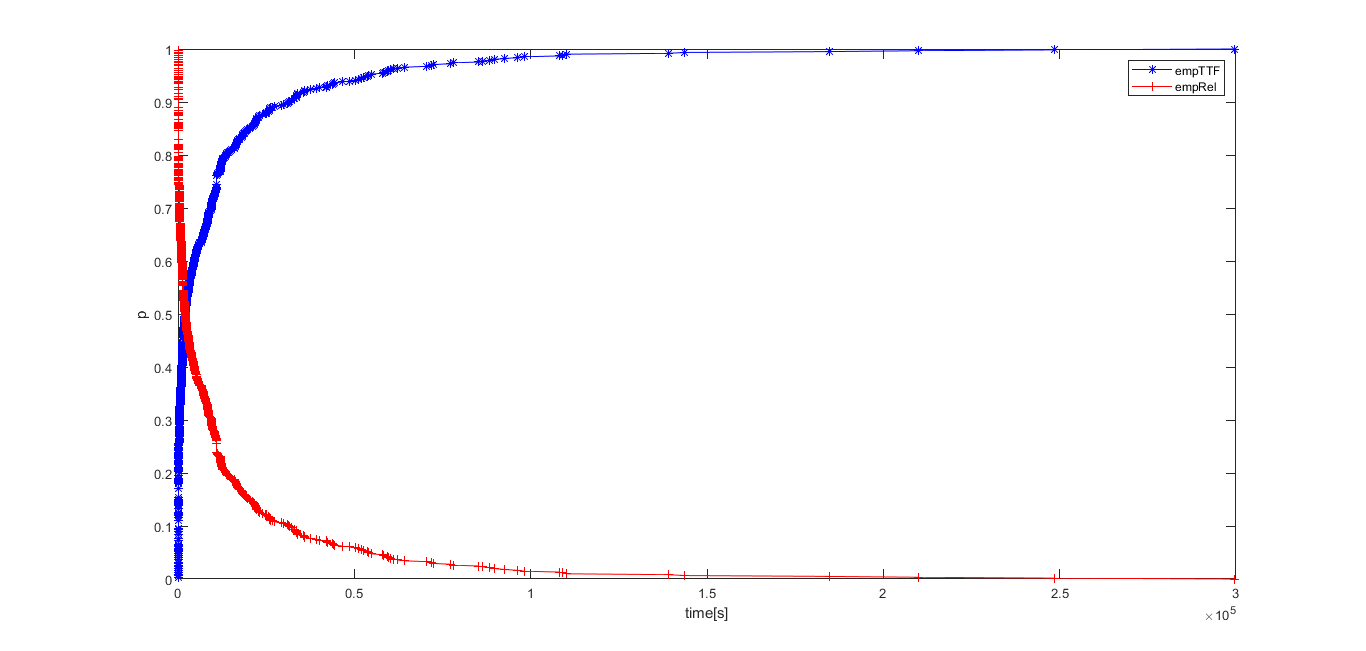
\includegraphics[width=\textwidth]{img/hw6/TTF_Mercury.png}
	\caption{\textit{Distribuzioni Empiriche Mercury}}
\end{figure}
\subsubsection{EmpTTF e EmpRel - BlueGene}
\begin{figure}[H]
	\centering
	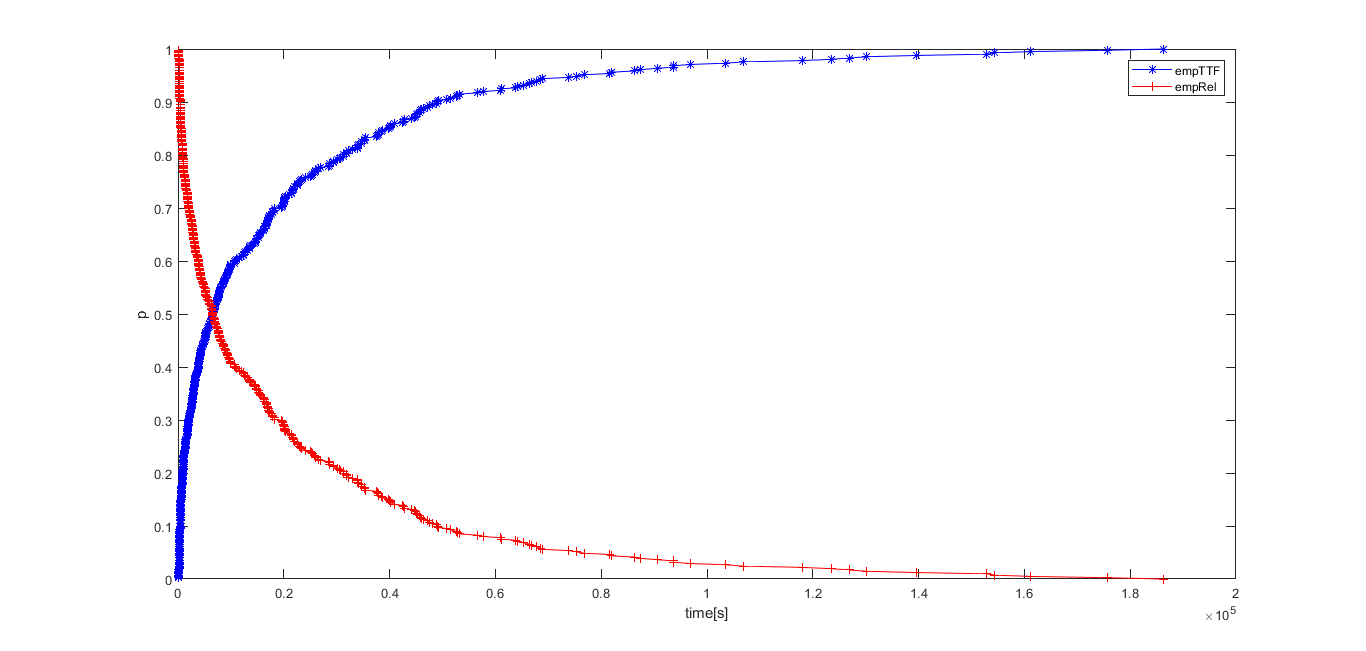
\includegraphics[width=\textwidth]{img/hw6/TTF_BG.png}
	\caption{\textit{Distribuzioni Empiriche Blue-Gene}}
\end{figure}
\subsection{Fitting di EmpRel}
Di tali distribuzioni opportunamente ottenute, bisogna effettuarne un \textit{Curve Fitting} in modo da ricavarne un modello statistico (così facendo ho informazioni anche sul probabile andamento futuro della curva). Tale operazione risulta essere fondamentale, in quanto una data distribuzione può essere sintomatica di un particolare guasto.
\\A tale scopo è stato utilizzato il tool MATLAB \textit{Curve Fitting}.
\subsubsection{Fitting EmpRel - Mercury}
Il fitting è stato eseguito con una distribuzione Esponenziale a 2 termini, descritta dalla seguente equazione:
\begin{equation*}
	f(x) = a*e^{bx}+c*e^{dx}
\end{equation*}
i cui coefficienti sono stati determinati tramite algoritmi interni del tool.
\begin{figure}[H]
	\centering
	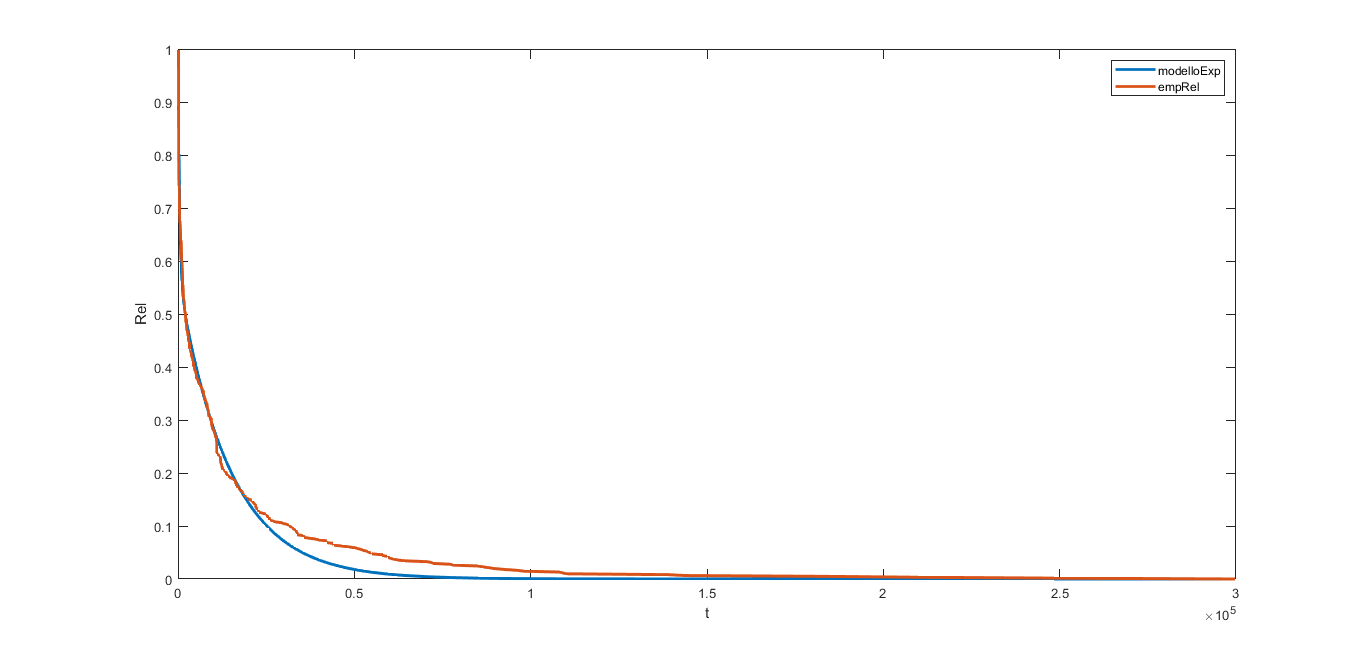
\includegraphics[width=\textwidth]{img/hw6/FittingM.png}
	\caption{\textit{Fitting empRel Mercury con distribuzione Esponenziale}}
\end{figure}
Tale analisi ha prodotto i seguenti risultati:
\begin{equation*}
	\begin{split}
		&SSE = 0,4685\\
		&Rsquare = 0,9872
	\end{split}
\end{equation*}
L' \textit{Rsquare} è un valore abbastanza elevato, a dimostrazione del fatto che la distribuzione esponenziale selezionata spiega gran parte della variazione di quella oggetto del fitting.
\\Come ulteriore dimostrazione della \textit{GOF - Goodness of Fit} è stato eseguito il già precedentemente citato \textit{Kolmogorov-Sminrov test}, il quale ha prodotto come risultato h = 0, verificando l'ipotesi nulla.
\begin{minted}[framesep = 1mm,
	fontsize = \footnotesize,
	breaklines,
	]{MATLAB}
	h = kstest2(empRel,fittedmodel(t));
\end{minted}
\subsubsection{Fitting EmpRel - BlueGene}
Lo stesso procedimento descritto in precedenza è stato iterato per il supercalcolatore Blue-Gene. Anche in questo caso è stata selezionata una distribuzione Esponenziale a 2 termini, come modello che meglio approssima la Reliability empirica del sistema.
\begin{figure}[H]
	\centering
	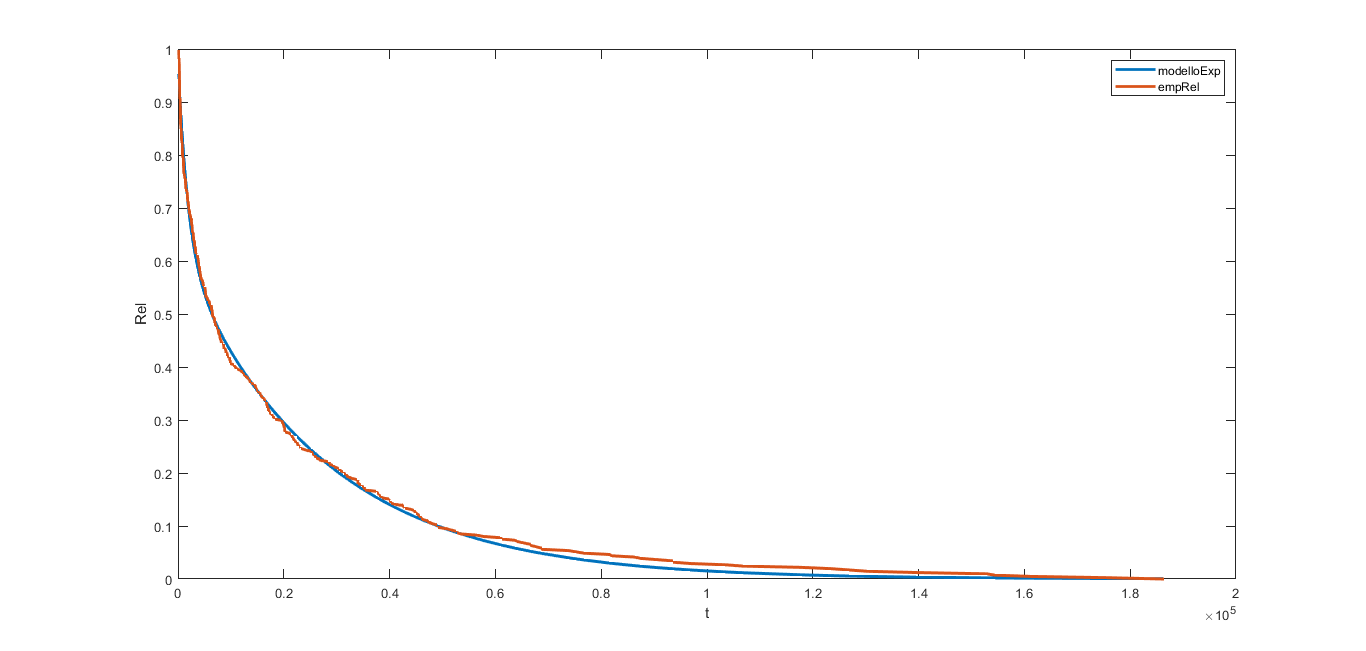
\includegraphics[width=\textwidth]{img/hw6/FittingBG.png}
	\caption{\textit{Fitting empRel Blue-Gene con distribuzione Esponenziale}}
\end{figure}
I risultati prodotti dall'analisi sono i seguenti:
\begin{equation*}
	\begin{split}
		&SSE = 0,08606\\
		&Rsquare = 0,9974
	\end{split}
\end{equation*}
Anche in questo caso il kstest ha fornito output h=0, confermando la bontà del fitting eseguito.
\\
La distribuzione esponenziale è associata a fenomeni degenerativi di tipo hardware (boh vedi meglio ste conclusioni - non sono convita che mercury sia esponenziale SSE non piccolo).
\subsection{Analisi Reliability per Sottocomponenti}
Sono stati eseguiti dei confronti tra Reliability dell'intero sistema e quella relativa ad alcuni dei suoi sottocomponenti, suddivisi per tipologia di nodo. 
\subsubsection{Mercury}
Per ogni categoria di nodo (master, login, computation e storage), sono stati selezionati quelli in cui, in base al report, è stato riscontrato il numero più elevato di fallimenti, effettuando quindi dei confronti "al limite":
\begin{itemize}
	\item \textbf{tg-master},
	\item \textbf{tg-login3},
	\item \textbf{tg-c401},
	\item \textbf{tg-s044}
\end{itemize}
Le entries associate a ciascuno di questi nodi sono state isolate in log specifici, i quali sono stati manipolati con le tecniche già descritte per i log principali. Per tutti i nodi è stata selezionata una finestra temporale di 150. Dopodichè, dagli interarrivi relativi ai singoli nodi sono state calcolate le Reliability Empiriche.
\\
\begin{figure}[H]
	\centering
	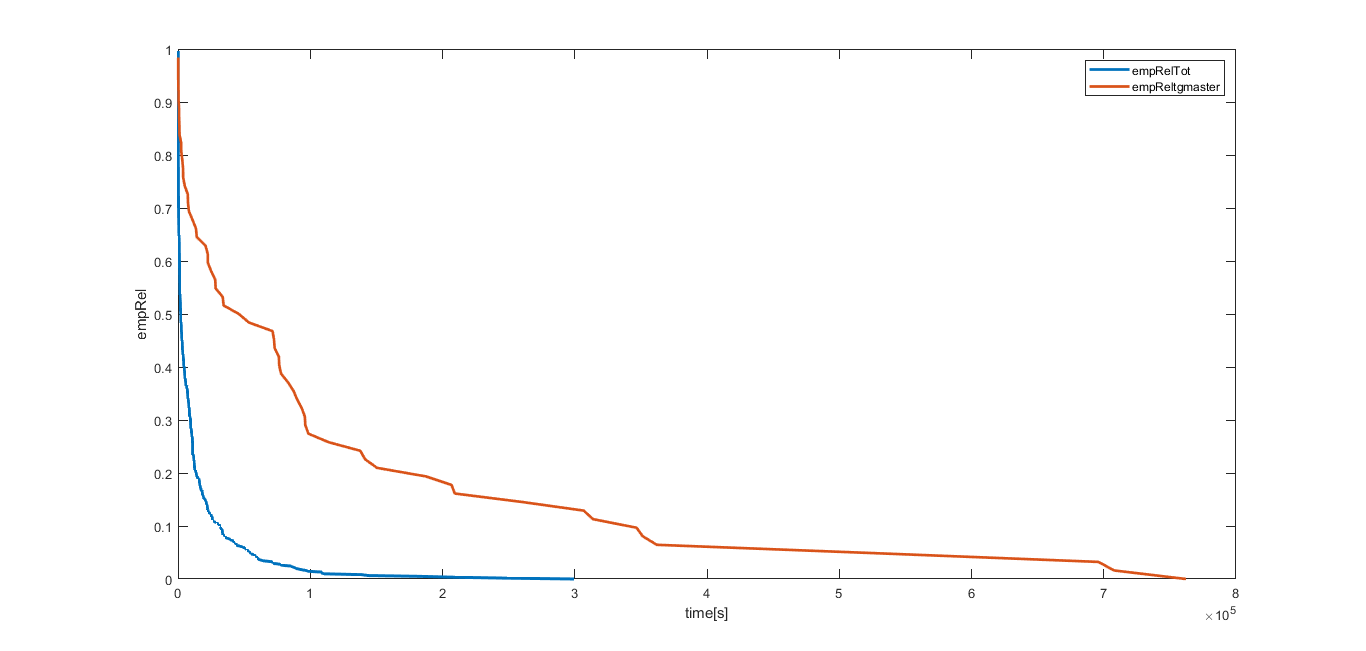
\includegraphics[width=\textwidth]{img/hw6/Rel_Tot_Tgmaster.png}
	\caption{\textit{Confronto Reliability Totale - Reliability tg-master}}
\end{figure}
\begin{figure}[H]
	\centering
	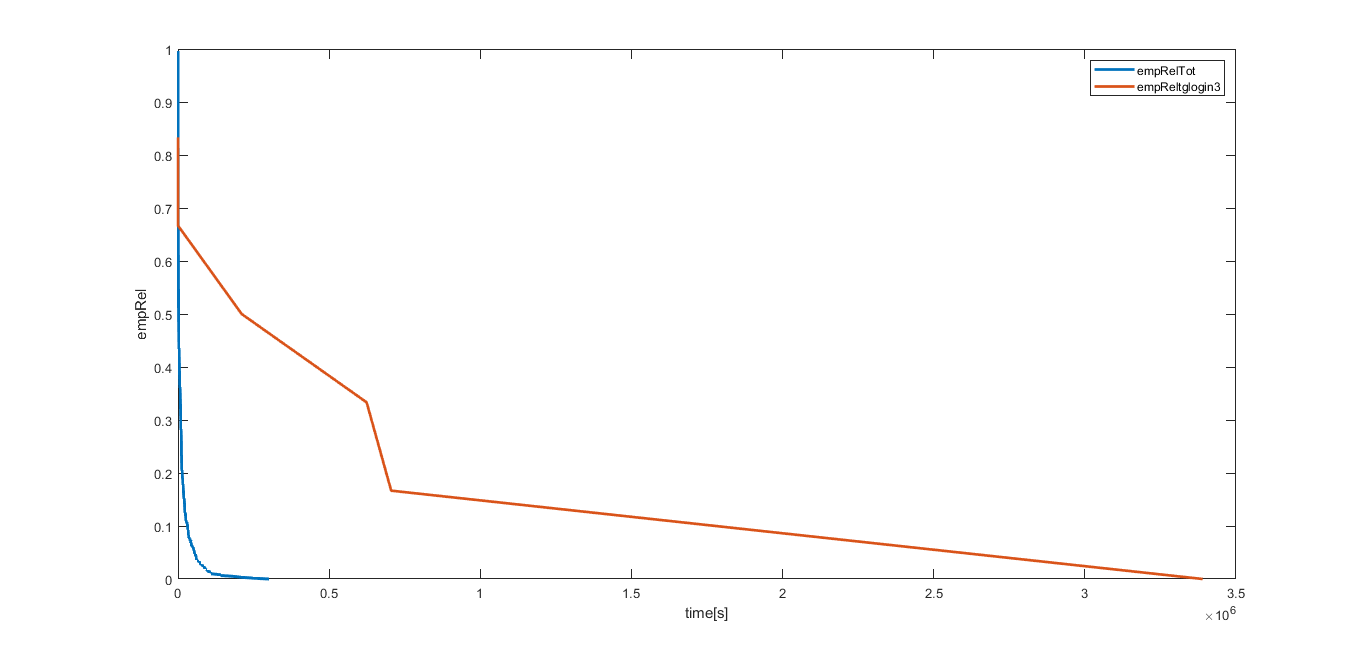
\includegraphics[width=\textwidth]{img/hw6/Rel_Tot_Tglogin.png}
	\caption{\textit{Confronto Reliability Totale - Reliability tg-login3}}
\end{figure}
\begin{figure}[H]
	\centering
	\includegraphics[width=\textwidth]{img/hw6/Rel_Tot_Tgc.png}
	\caption{\textit{Confronto Reliability Totale - Reliability tg-c401}}
\end{figure}
\begin{figure}[H]
	\centering
	\includegraphics[width=\textwidth]{img/hw6/Rel_Tot_Tgs.png}
	\caption{\textit{Confronto Reliability Totale - Reliability tg-s044}}
\end{figure}
Quindi tutti i nodi eccetto il tg-c401, hanno una reliability migliore rispetto a quella totale del sistema. 
\\Il nodo di computation \textbf{tg-c401} per tempi brevi in confronto ai totali, risulta essere il meno reliable, addirittura anche rispetto al sistema. Ciò significa che esso potrebbe essere un probabile collo di bottiglia per il supercalcolatore Mercury. Quest'ultima affermazione è molto probabile in quanto tale nodo è quello caratterizzato dal maggior numero di fallimenti.
\\In seguito è stato riportato un grafico che confronta tra di loro le reliability dei diversi nodi selezionati:
\begin{figure}[H]
	\centering
	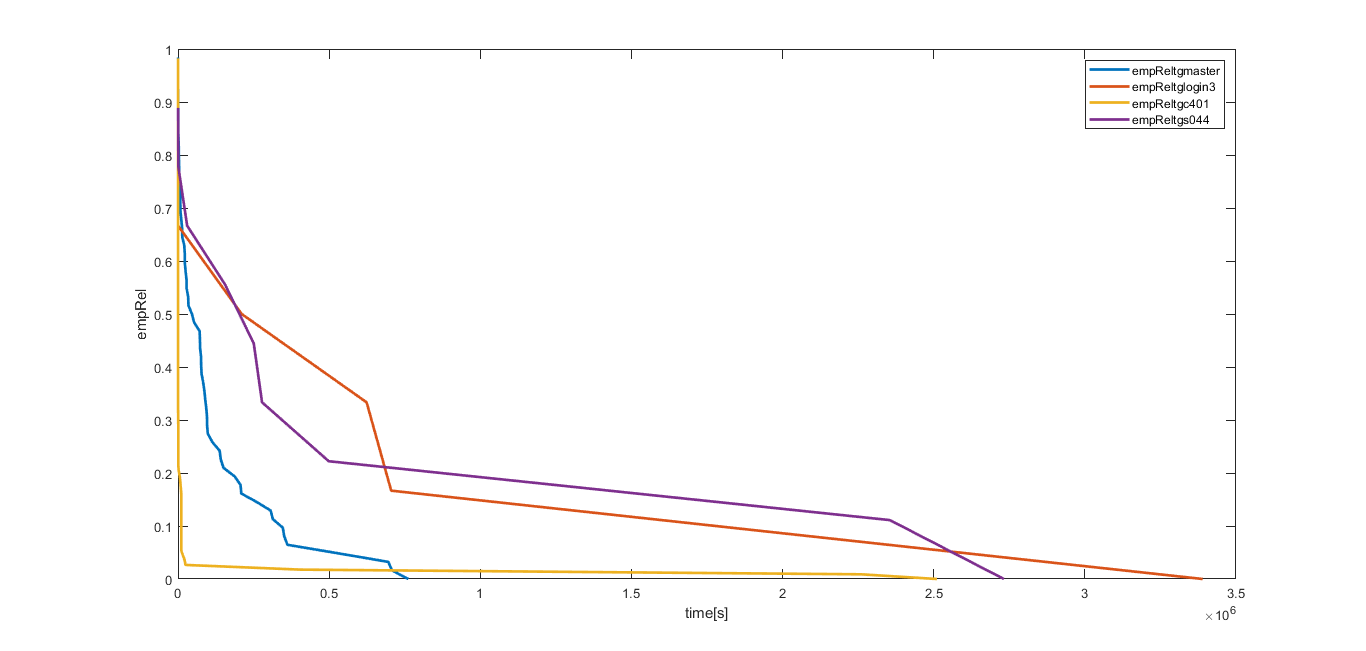
\includegraphics[width=\textwidth]{img/hw6/confrontoMercury.png}
	\caption{\textit{Confronto Reliability Nodi Mercury}}
\end{figure}
Altre considerazioni su quest'ultima immagine pensaci dopo.
\\
\\
Un altro confronto è stato effettuato sulla reliability di nodi funzionalmente simili tra di loro.
\\Per tale analisi sono stati selezionati tre nodi computation:
\begin{itemize}
	\item \textbf{tg-c401}, il nodo con il numero maggiore di fallimenti,
	\item \textbf{tg-c238},
	\item \textbf{tg-c242}.
\end{itemize}
Gli ultimi due presentano un numero di fallimenti molto simile tra di loro.
\begin{figure}[H]
	\centering
	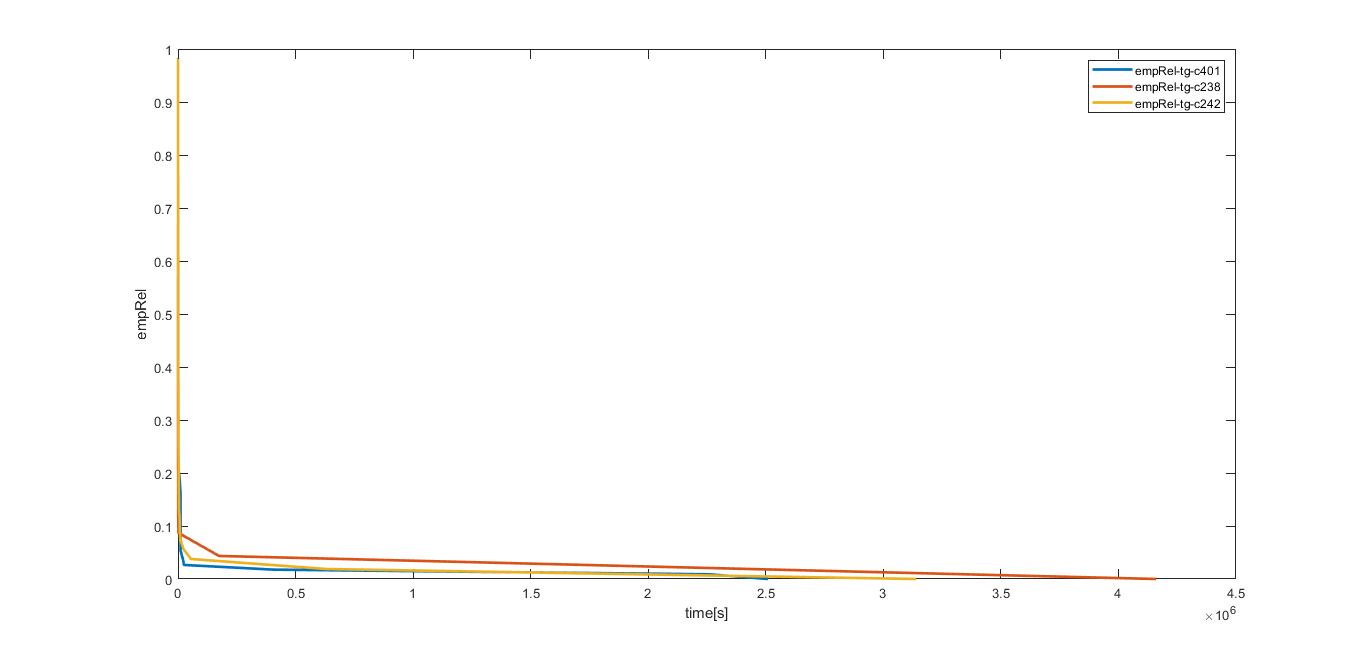
\includegraphics[width=\textwidth]{img/hw6/RelCompMercury.png}
	\caption{\textit{Confronto Reliability Nodi Computation Mercury}}
\end{figure}
La reliability del nodo 401 risulta essere sempre peggiore delle altre, anche se nonostante ciò gli andamenti risultano essere tutti molto simili tra di loro (rispettivamente 1273 e 1067). Tutti i nodi computation analizzati hanno dunque una reliability molto bassa.
\subsubsection{Blue-Gene}
L'analisi è stata ripetuta anche per i primi 3 nodi con più entries di fallimenti di Blue-Gene. Essi, ordinati per numero di entries, sono:
\begin{itemize}
	\item \textbf{R71-M0-N4},
	\item \textbf{R12-M0-N0},
	\item \textbf{R63-M0-N2}
\end{itemize} 
\begin{figure}[H]
	\centering
	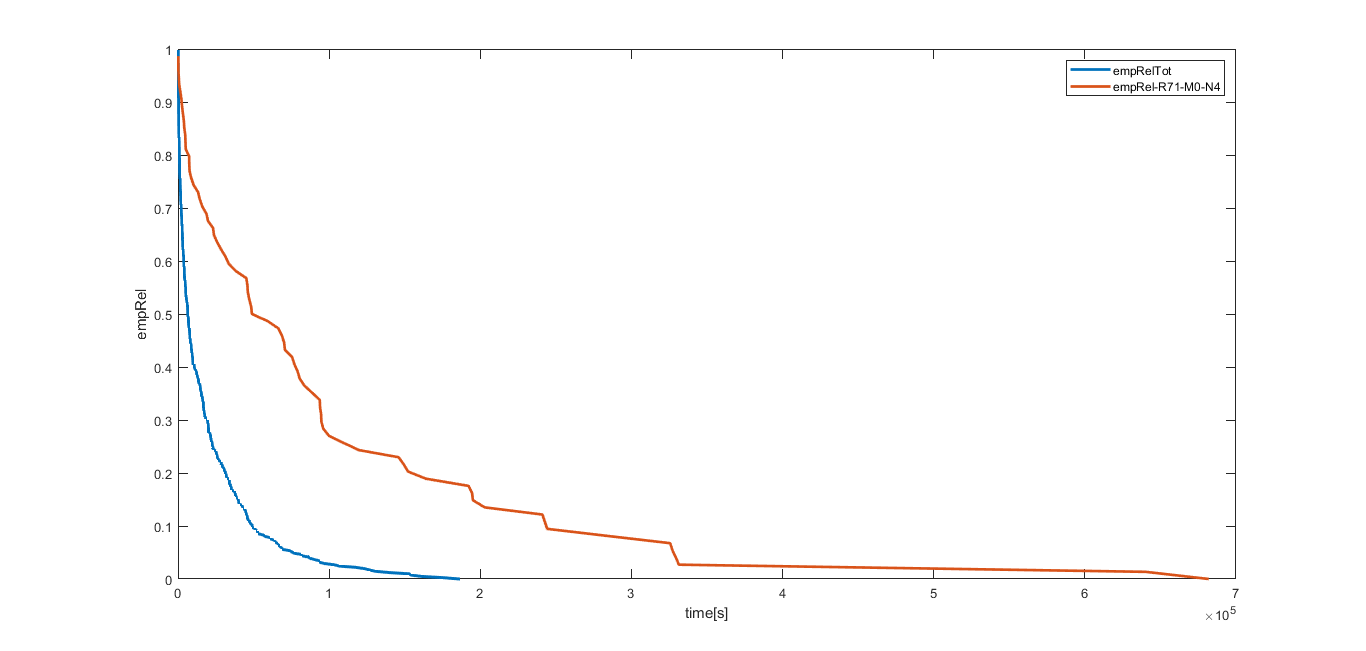
\includegraphics[width=\textwidth]{img/hw6/Rel_Tot_R71.png}
	\caption{\textit{Confronto Reliability Totale - Reliability R71-M0-N4}}
\end{figure}
\begin{figure}[H]
	\centering
	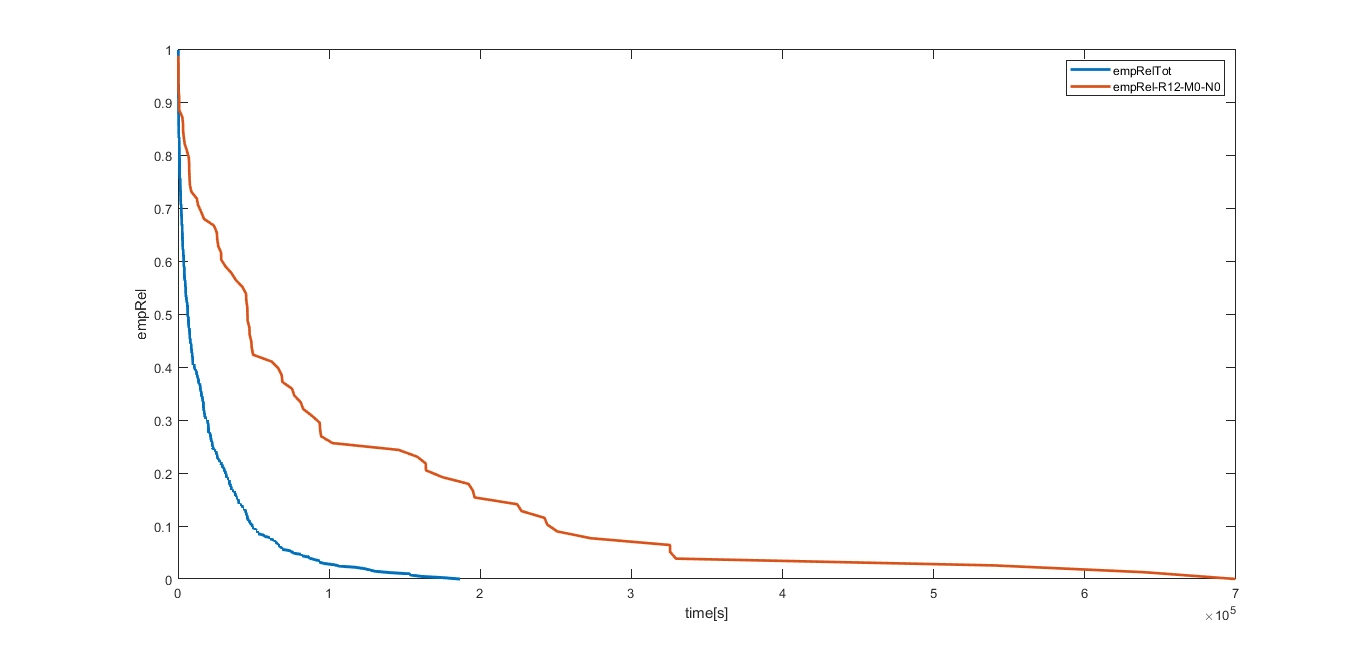
\includegraphics[width=\textwidth]{img/hw6/Rel_Tot_R12.png}
	\caption{\textit{Confronto Reliability Totale - Reliability R12-M0-N0}}
\end{figure}
\begin{figure}[H]
	\centering
	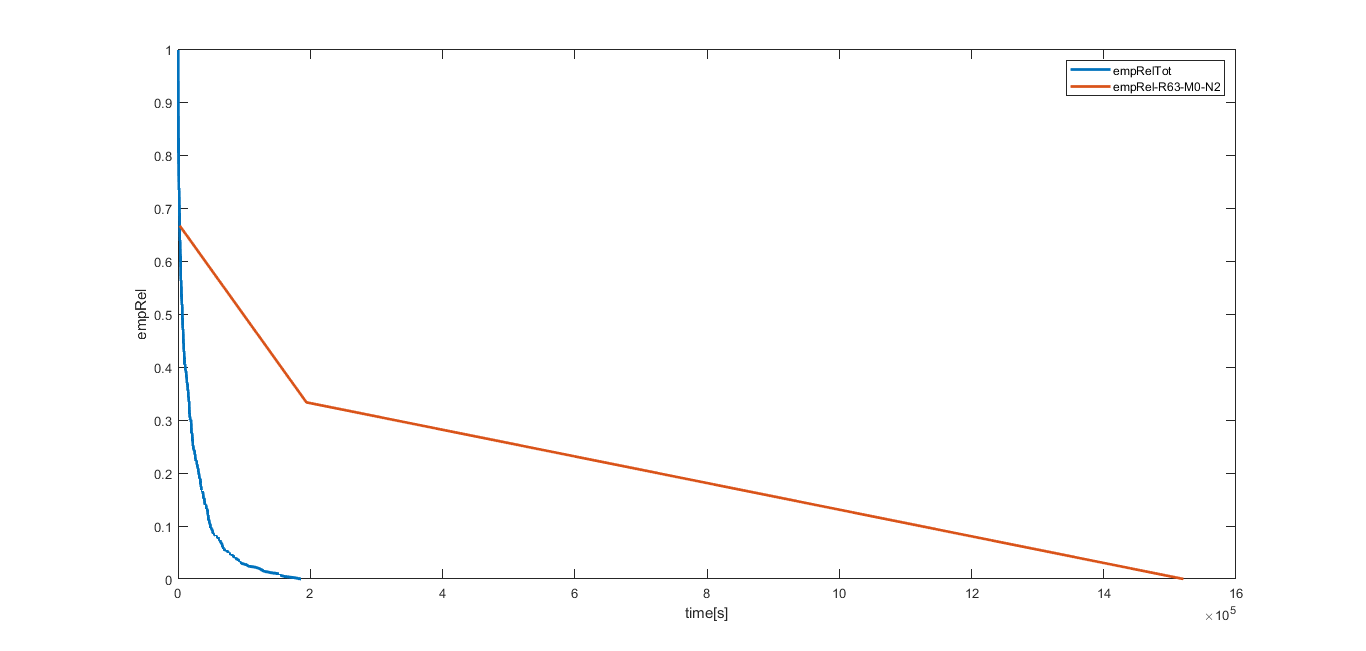
\includegraphics[width=\textwidth]{img/hw6/Rel_Tot_R63.png}
	\caption{\textit{Confronto Reliability Totale - Reliability R63-M0-N2}}
\end{figure}
In tal caso non risultano esserci evidenti colli di bottiglia, e la reliability del singolo nodo risulta essere sempre maggiore di quella totale del sistema.
\\Anche per Blue-Gene si riporta un grafico in cui vengono messe a confronto le reliability dei 3 differenti nodi:
\begin{figure}[H]
	\centering
	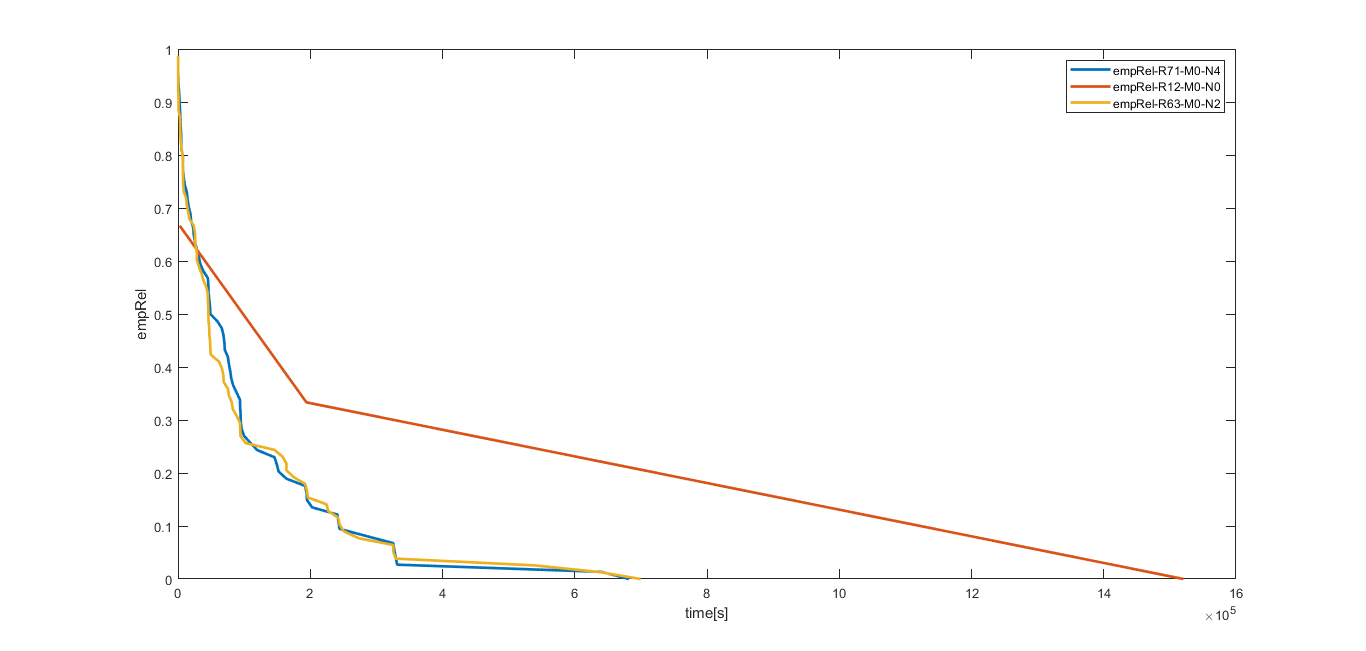
\includegraphics[width=\textwidth]{img/hw6/confrontoBG.png}
	\caption{\textit{Confronto Reliability Nodi Blue-Gene}}
\end{figure}
In tal caso i nodi confrontati sono tutti funzionalmente simili. Come si evince dal grafico la reliability del nodo \textbf{R71-M0-N4} e \textbf{R63-M0-N2} risulta avere un andamento molto simile, a differenza del terzo nodo il quale è più reliable dei precedenti.
\subsection{Domanda 5}
Esiste una relazione tra tipo di errore e nodo(mercury)?

